% Propietario conservado: /Users/ruben/Documents/New project/output/REVISION_ARGUMENTAL_APERTURAS_CIERRES_20260915/VI/delivery/MANUSCRIPT_VI_ES_EN_COMPLETE/source_es/sections/04_atlas_familias.tex
\section{Classification of persistent sections and their internal observables}
\label{vi:vi:sec:atlas}

Classification begins with the support on which transport acts.
Physical names are interpreted after its invariants have been constructed.
This priority distinguishes a position, a history, and a species:
the position belongs to the finite atlas; the history preserves the transitions
producing it; the persistence type gathers histories compatible with the
same classification. An evaluated mass is a subsequent reading of that object.

\subsection{Parity, depth, and multisections}

On the positional copy of APP, consider
\[
 I_9=\{1,\ldots,9\},\qquad \mathcal C=I_9\times I_9.
\]
The ordered pair preserves the two axes. Define the parity classifier
\[
 f(r,c)=
 \begin{cases}
 \ell,&r,c\text{ odd},\\
 \nu,&r\text{ odd},\ c\text{ even},\\
 d,&r\text{ even},\ c\text{ odd},\\
 u,&r,c\text{ pairs},
 \end{cases}
 \qquad g(r,c)=\max\{|r-5|,|c-5|\}.
\]
The symbols of the first map initially name internal classes.
The second measures combinatorial depth relative to the centre. Subsequent
association with physical sectors must preserve these definitions.


% BEGIN OWNER /Users/ruben/Documents/New project/output/REVISION_ARGUMENTAL_APERTURAS_CIERRES_20260915/VI/delivery/MANUSCRIPT_VI_ES_EN_COMPLETE/source_es/figures/atlas_clasificacion.tex
\begin{figure}[H]
\centering
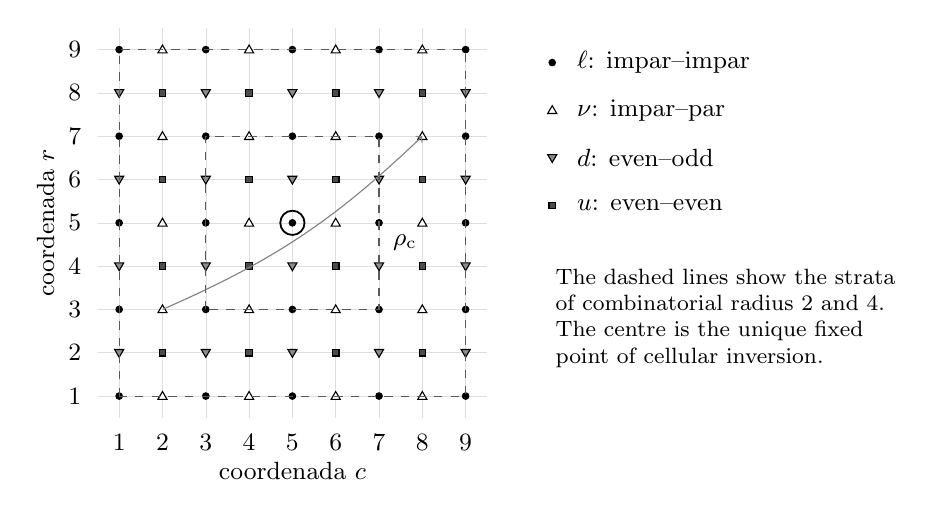
\begin{tikzpicture}[x=.55cm,y=.55cm, every node/.style={font=\small}]
  \draw[step=1,black!13,very thin] (.5,.5) grid (9.5,9.5);
  \foreach \k in {1,...,9} {
    \node[below] at (\k,.35) {$\k$};
    \node[left] at (.35,\k) {$\k$};
  }
  \node[below] at (5,-.3) {coordenada $c$};
  \node[rotate=90] at (-.7,5) {coordenada $r$};
  \foreach \r in {1,...,9} {
    \foreach \c in {1,...,9} {
      \pgfmathtruncatemacro{\pr}{mod(\r,2)}
      \pgfmathtruncatemacro{\pc}{mod(\c,2)}
      \ifnum\pr=1
        \ifnum\pc=1
          \draw[fill=black] (\c,\r) circle (.075);
        \else
          \draw[fill=white] (\c,\r+.105)--(\c-.105,\r-.075)--(\c+.105,\r-.075)--cycle;
        \fi
      \else
        \ifnum\pc=1
          \draw[fill=black!45] (\c,\r-.105)--(\c-.105,\r+.075)--(\c+.105,\r+.075)--cycle;
        \else
          \draw[fill=black!70] (\c-.075,\r-.075) rectangle (\c+.075,\r+.075);
        \fi
      \fi
    }
  }
  \draw[black!65,dashed] (3,3) rectangle (7,7);
  \draw[black!65,dashed] (1,1) rectangle (9,9);
  \draw[line width=.65pt] (5,5) circle (.28);
  \draw[->,black!50] (2,3) to[bend right=10] (8,7);
  \node[fill=white,inner sep=2pt] at (7.6,4.55) {$\rho_{\mathrm c}$};
  \begin{scope}[shift={(11,8.7)}]
    \draw[fill=black] (0,0) circle (.075);
    \node[right] at (.35,0) {$\ell$: impar--impar};
    \draw[fill=white] (0,-.995)--(-.105,-1.175)--(.105,-1.175)--cycle;
    \node[right] at (.35,-1.1) {$\nu$: impar--par};
    \draw[fill=black!45] (0,-2.305)--(-.105,-2.125)--(.105,-2.125)--cycle;
    \node[right] at (.35,-2.2) {$d$: even--odd};
    \draw[fill=black!70] (-.075,-3.375) rectangle (.075,-3.225);
    \node[right] at (.35,-3.3) {$u$: even--even};
    \node[anchor=west,text width=4.4cm,align=left,font=\footnotesize]
      at (-.15,-5.9) {The dashed lines show the strata of combinatorial radius $2$ and $4$. The centre is the unique fixed point of cellular inversion.};
  \end{scope}
\end{tikzpicture}
\caption[Classification on the positional atlas]{Classification on the positional atlas. The marks distinguish the
four internal parity classes, preceding their physical realisations.
Depth is measured by $g(r,c)=\max(|r-5|,|c-5|)$.
The arrow illustrates $(2,3)\mapsto(8,7)$ under cellular inversion;
it does not represent a dynamic trajectory or a change of flavour.
The central circle marks $(5,5)$, at depth zero.}
\label{vi:vi:fig:atlas}
\end{figure}

% END OWNER


\begin{definition}[Family and depth multisection]
For every realised pair \(y=(f,g)\), define
\[
 \mathfrak S_y=\{(r,c)\in\mathcal C:(f(r,c),g(r,c))=y\}.
\]
Its lift to persistent states is the preimage under the projection
onto the atlas, preserving the sheets, orientations, and memory of the extension.
\end{definition}

\begin{proposition}[Census of the multisections]
\label{vi:vi:prop:censo13}
The atlas contains \(81\) cells and exactly \(13\) nonempty multisections.
Their distribution is
\[
\begin{array}{c|c|c|r}
\text{class}&\text{depths}&\text{cardinals}&\text{total}\\\hline
\ell&0,2,4&1,8,16&25\\
\nu&1,2,3,4&2,4,6,8&20\\
d&1,2,3,4&2,4,6,8&20\\
u&1,3&4,12&16
\end{array}
\]
\end{proposition}
\begin{proof}
In \(I_9\) there are \(5\) odd and \(4\) even numbers. The four classes have
cardinalities \(25,20,20,16\). For the odd--odd class, the centred squares
of radii \(0,2,4\) contain \(1,9,25\) points; the
differences are \(1,8,16\). For odd--even, the cumulative rectangles
at radii \(1,2,3,4\) contain \(2,6,12,20\) points, whose
differences are \(2,4,6,8\). Interchanging the axes proves the
even--odd case. In even--even there are \(4\) points through radius \(1\) and \(16\)
through radius \(3\), so the strata have \(4,12\) points.
The sets are disjoint, and their union is \(\mathcal C\).
\end{proof}

This census explains the meaning of each cardinality before any particle
table. Depth \(g\) is not by itself identified with the index of a
physical generation either: that identification uses the realisation
maps of the corresponding sector.

\subsection{Central conjugation and selection of a cell}

Cellular inversion is
\[
 \rho_{\mathrm c}(r,c)=(10-r,10-c).
\]
It preserves parity and depth and therefore acts within every
multisection. Its unique fixed point satisfies \(2r=2c=10\): it is \((5,5)\).
The remaining \(80\) cells are grouped into \(40\) pairs. There are thus
\(41\) orbits, only one of which is a singleton.

\begin{proposition}[Obstruction to noncentral point selection]
If a cell selector is required to depend only on the family--depth pair
and to be equivariant for \(\rho_{\mathrm c}\), it can exist
only in the central multisection.
\end{proposition}
\begin{proof}
Inversion acts trivially on the pair \(y\). Equivariance of
\(a(y)\in\mathfrak S_y\) requires
\(a(y)=a(\rho_{\mathrm c}y)=\rho_{\mathrm c}a(y)\).
Thus \(a(y)\) would have to be the unique fixed point \((5,5)\).
In the central multisection, this is precisely the available choice.
\end{proof}

The consequence is structural. The treatment of the electron by means of a
fiber of rank \(1\) does not authorize treating all the other
families in this way. Outside the center, the orbit, the multisection and the orientations
it preserves belong to the object being evaluated.

\subsection{Classification of routes and positional memory}

The chronological chart assigns to each cell the sextuple
\[
 \mathcal R(r,c)=
 (n_A,s_C,k_{\Delta_4},b_{120},b_{\zeta},\tau_{12})_{r,c}.
\]
The five integer coordinates come from the oriented record; the last
preserves the dodecaphasic word. Two cells belong to the same route
family when these six readings coincide. This is a quotient different
from the family--depth quotient.

In the documented finite census of this chart, \(56\) families appear.
The size histogram is
\[
 41\times1,\quad10\times2,\quad2\times3,\quad1\times4,\quad2\times5.
\]
The identities
\[
 41+10+2+1+2=56,\qquad
 41+20+6+4+10=81
\]
check the number of classes and coverage of the support. Reproducing
the census requires the sextuples produced by transport, not merely these
two sums. The data dossier preserves the \(81\) rows and the
\(56\) complete classes.

Fixing the lexicographic order in each fibre, let \(\kappa_{\mathrm{pos}}\)
be the rank of the cell. Then
\[
 (r,c)\longmapsto\bigl(\mathcal R(r,c),\kappa_{\mathrm{pos}}(r,c)\bigr)
\]
is injective. \(5\) positional-memory values are required because
fibres of size \(5\) exist; the pigeonhole principle rules out a
uniform injective lift with fewer values. This memory is neither colour
nor the mass exponent, although all subsequently enter the same history.

\subsection{Residual colour, flavour, and sheets}

In the \(36\) cells with even first coordinate, the residual-colour
observable is defined by
\[
 \operatorname{col}(r,c)=r-c\pmod3.
\]
For each even \(r\), the \(9\) values of \(c\) traverse each class
\(3\) times. This gives the exact distribution
\[
 36=12+12+12.
\]
Central inversion transforms this observable into its opposite, since
\[
 (10-r)-(10-c)=-(r-c).
\]
It fixes class \(0\) and interchanges \(1\) and \(2\). The colour
representation subsequently uses this ternary support and its operators;
the number of residues does not replace construction of the representation.

Flavour distinguishes classes and realisations of the sector, whereas residual
colour distinguishes positions within the corresponding ternary support.
The sheet, by contrast, identifies the arithmetic evaluation entering
a transition. Sheet interchange acts on a history; it is not
an operation that renames flavour. This distinction allows
mixing, conjugation, and mass evaluations to be formulated
separately.

\subsection{Domain of orientations of the atlas}

Each cell admits \((h,v)\in\{\pm1\}^2\), so that
\[
 \mathcal C^{\mathrm{or}}=\mathcal C\times\{\pm1\}^2,
 \qquad |\mathcal C^{\mathrm{or}}|=324.
\]
The canonical orientation of \(81\) routes and the full domain of \(324\)
are two distinct domains. A reader can descend to a family in the
first chart and cease to be constant when the four
orientations are considered. Therefore, each statement about the coincidence of readers
identifies its domain before publishing the census.

The finite structure therefore combines positions, route families,
multisections, conjugation orbits and residual observables. None
of these partitions replaces the others. The following mass development
acts on their persistent lifts, retaining the information that
each evaluation needs.
